\chapter{Технологический раздел}
\section{Разработанные микросервисы}
В данную систему включены пять микросервисов:
\begin{itemize}
    \item \verb|scout|~--- поиск новостных лент с feedly.com;
    \item \verb|raider|~--- мониторинг новостей;
    \item \verb|soothsayer|~--- мониторинг экспертной оценки с сайта stopfake.org;
    \item \verb|compounder|~--- кластеризация новостей;
    \item \verb|rater|~--- ранжирование источников;
\end{itemize}

\section{Брокер сообщений и персистентное хранилище}
В данной работе принято решение использовать kafka в качестве такой системы, как наиболее развитой комбинации персистентного хранилища и брокера сообщений.

Рассмотрим подробнее принцип работы kafka. Кластер kafka обслуживает запросы от различных приложений, которые могут являться как потребителями сообщений, так и поставщиками (рис.~\ref{fig:kafka-apis}).

\begin{figure}[h]
    \centering
    \begin{subfigure}{.5\textwidth}
        \centering
        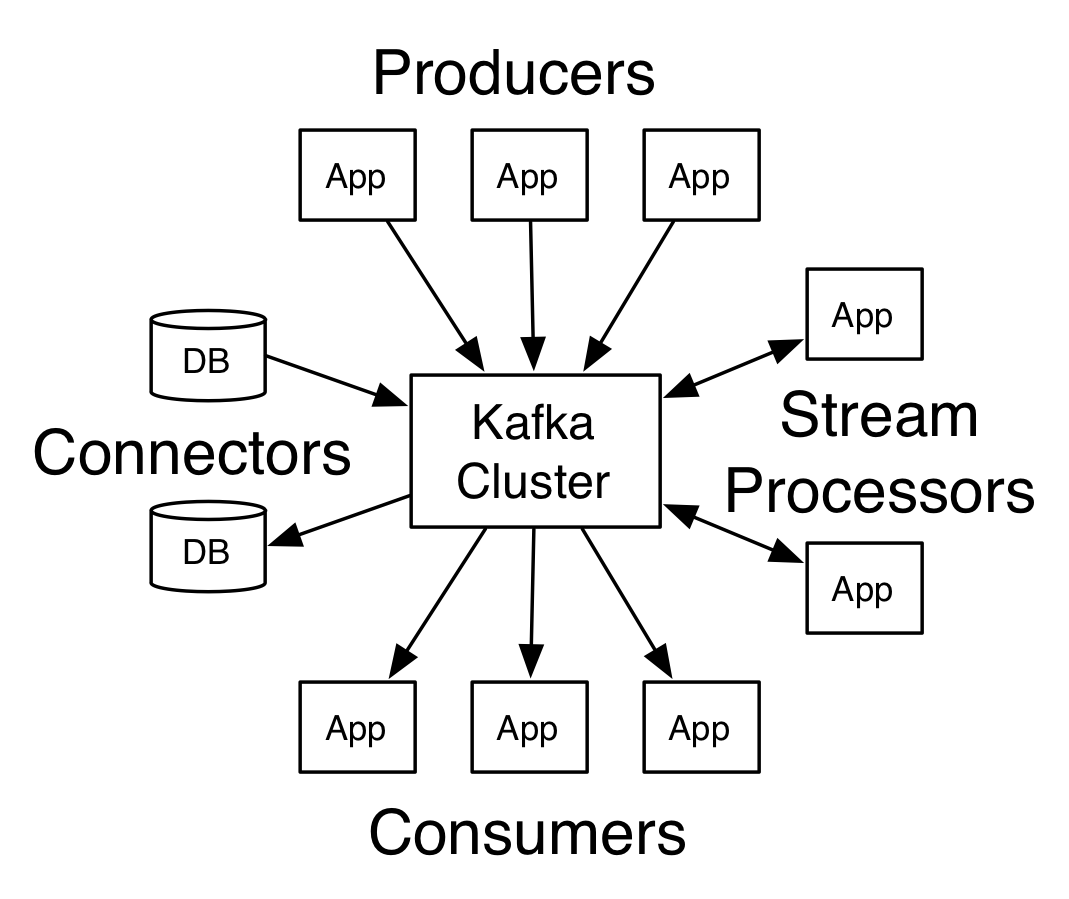
\includegraphics[width=\textwidth]{kafka-apis.png}
        \caption{Кластер kafka.}
        \label{fig:kafka-apis}
    \end{subfigure}%
    \begin{subfigure}{.5\textwidth}
        \centering
        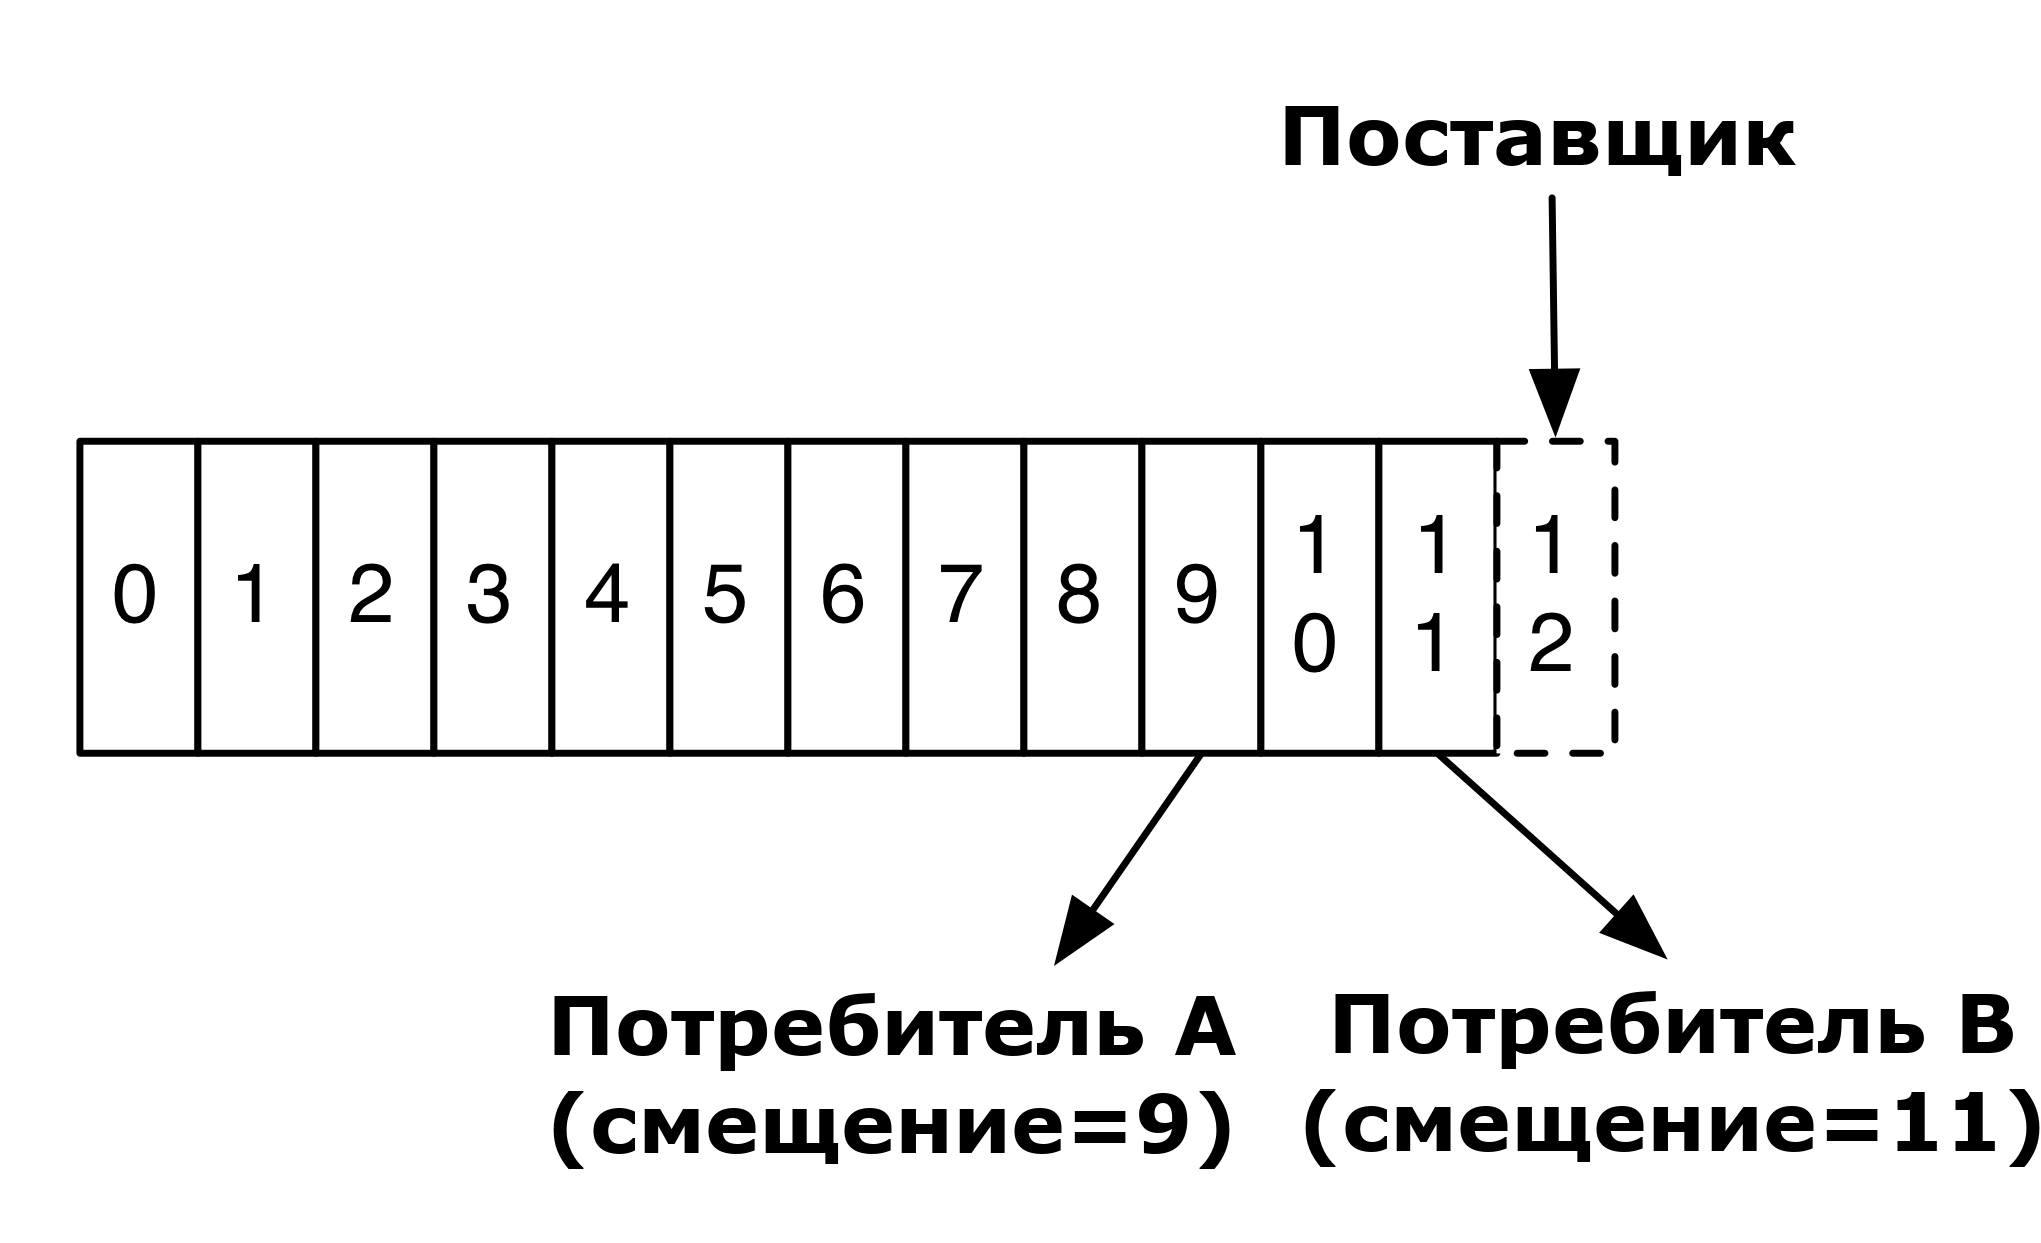
\includegraphics[width=\textwidth]{kafka-pubsub.png}
        \caption{Буфер темы с сообщениями.}
        \label{fig:kafka-pubsub}
    \end{subfigure}
    \caption{Apache Kafka.}
\end{figure}

Все хранилища данных, представленные на диаграмме потоков данных системы (рис.~\ref{fig:dataflows}) представляются как темы в терминах kafka. Каждая тема~--- буфер, хранящий все поступающие сообщения. Каждый потребитель получает сообщения по смещению в этом буфере (рис.~\ref{fig:kafka-pubsub}). Такой буфер полностью хранится на файловой системе, а производительность считывания достигается за счёт последовательного чтения и использования операционной системой файлового кеша.

Распределённость системы получается благодаря разделению буфера на несколько разделов \cite{wang12}, каждый из которых реплицируется внутри kafka кластера (рис.~\ref{fig:kafka-clusters}).

\begin{figure}[h]
    \centering
    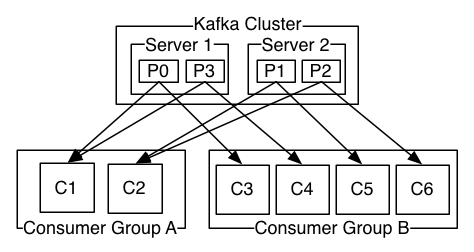
\includegraphics[width=.6\textwidth]{kafka-clusters.png}
    \caption{Репликация буферов внутри кластера kafka.}
    \label{fig:kafka-clusters}
\end{figure}

\section{Язык программирования и инструменты разработки}
Поставленная задача требует частого взаимодействия с подсистемой ввода-вывода: HTTP, работа с брокером сообщений. Из этого следует необходимость в асинхронной архитектуре микросервисов. Кроме того, основные микросервисы, для сбора новостей и кластеризации, требовательны к вычислительным ресурсам, поэтому необходимо использовать компилируемый язык программирования с производительностью сравнимой с Си. Также хотелось избежать накладных расходов на работу сборщика мусора. Поэтому в качестве языка программирования был выбран Rust.

В качестве редактора кода был использован NeoVim на ОС Arch Linux. Сборка проекта осуществляется пакетным менеджером cargo~--- стандартным инструментом для разработчиков на Rust. В качестве системы контроля версий использовался git.

Сама система запущена на серверах, предоставляемых digitalocean.com.

\section{Тестирование}
Для наиболее сложных компонентов, входящих в систему, реализовано модульное тестирование~--- тестирование отдельного модуля для проверки корректности его работы в штатных и исключительных ситуациях. Это позволяет достаточно быстро проверить, не привело ли очередное изменение кода к регрессии.

Наиболее требовательным к тестированию компонентом является модуль выделения основного содержимого из html-документа. Для тестирования данного модуля использовался набор системных тестов, разработанный сотрудниками mozilla для аналогичного модуля на js.

\section{Выводы}
Резюмируем список выбранных технологий:
\begin{itemize}
    \item Брокер сообщений: Apache Kafka;
    \item Персистентное хранилище: Apache Kafka;
    \item Язык программирования: Rust;
\end{itemize}
